% Figure 8: ResNet-110 Results
\begin{figure*}[t]
\centering
\begin{minipage}{0.48\textwidth}
  \centering
  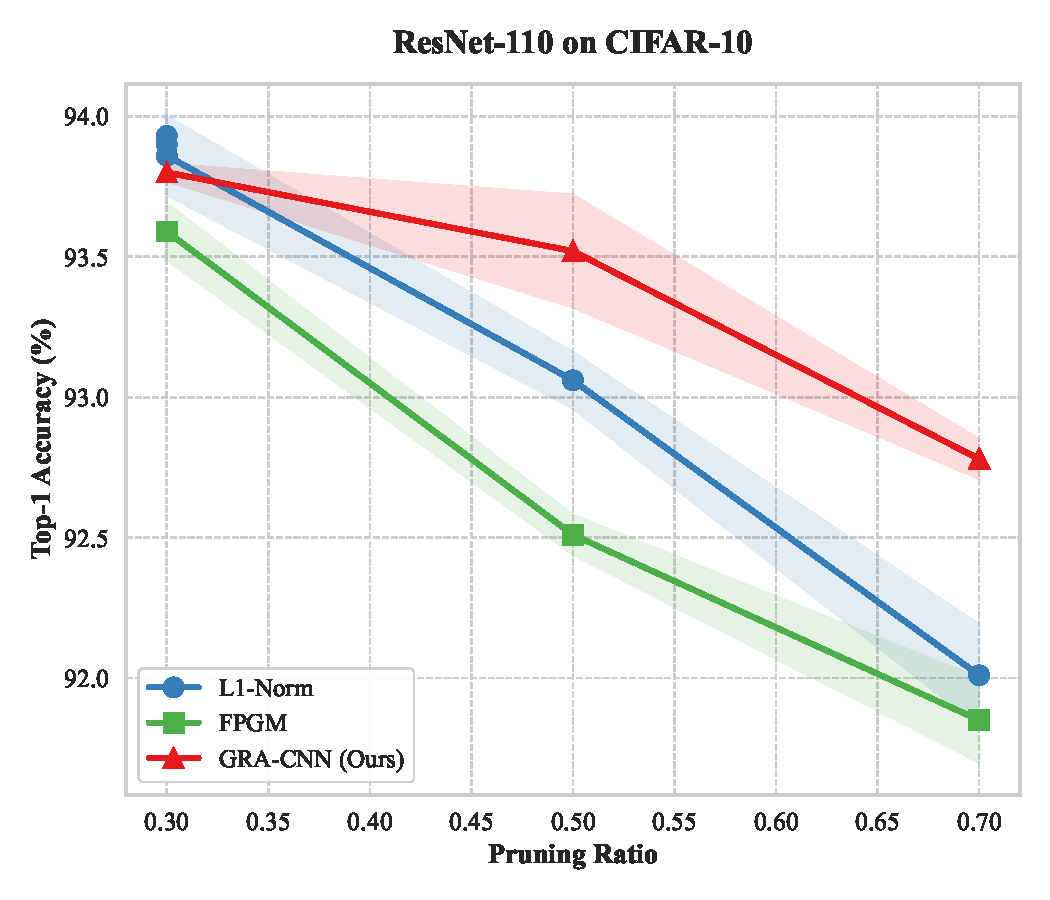
\includegraphics[width=\linewidth]{fig8_accuracy.pdf}
  \caption{Accuracy vs Pruning Ratio (ResNet-110)}
  \label{fig:res110_acc}
\end{minipage}
\hfill
\begin{minipage}{0.48\textwidth}
  \centering
  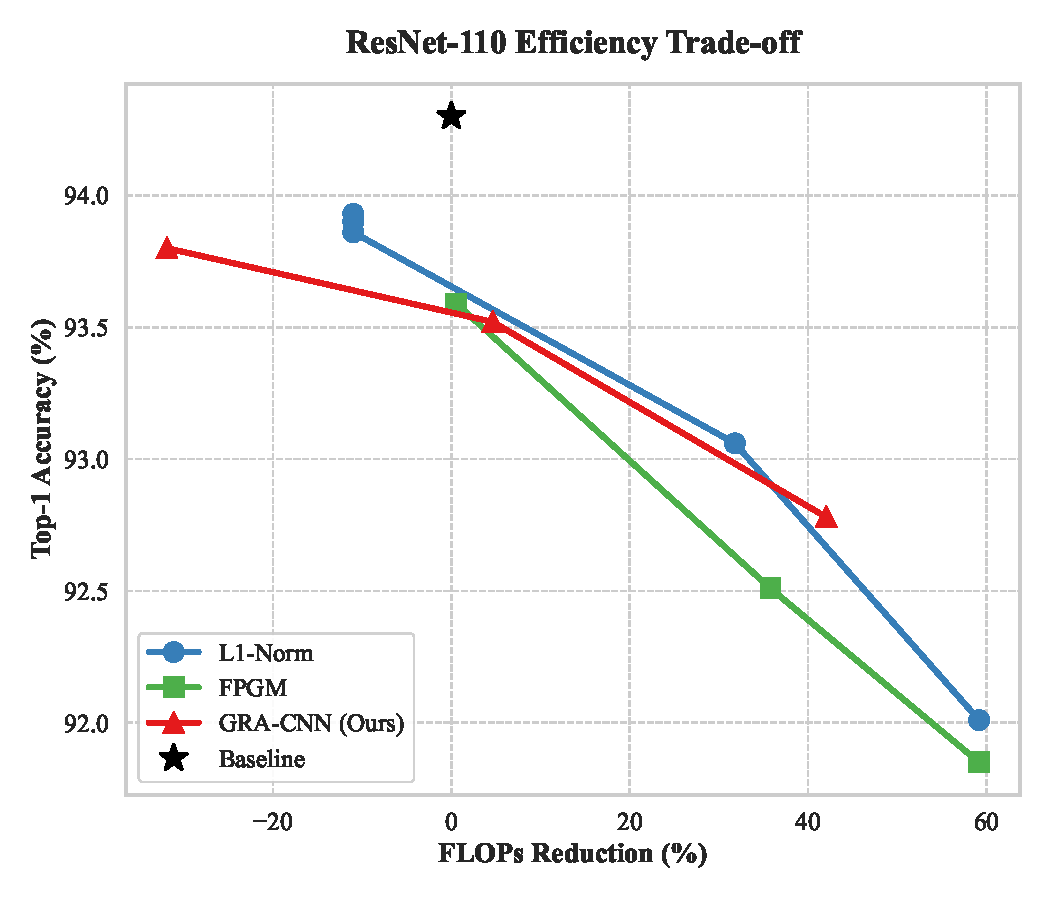
\includegraphics[width=\linewidth]{fig8_tradeoff.pdf}
  \caption{FLOPs Reduction vs Accuracy (ResNet-110)}
  \label{fig:res110_tradeoff}
\end{minipage}
\end{figure*}

% Figure 9: VGG-16 Results
\begin{figure*}[t]
\centering
\begin{minipage}{0.48\textwidth}
  \centering
  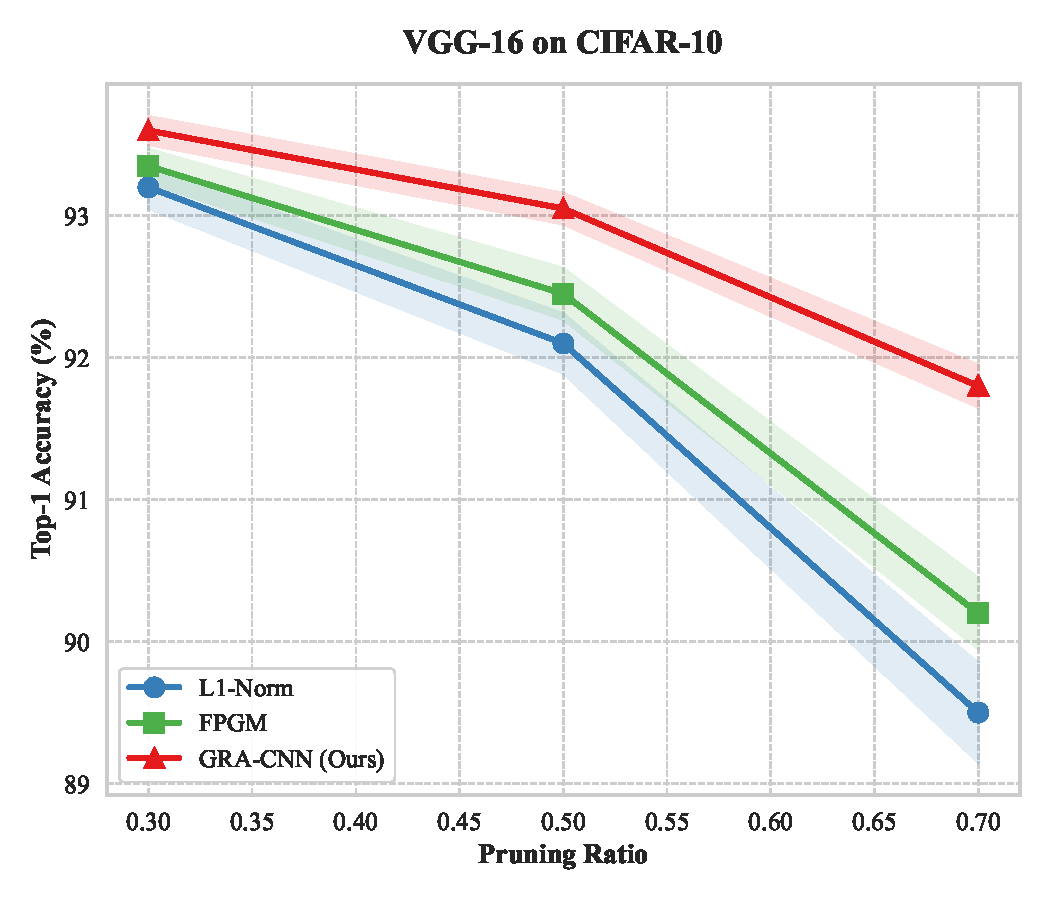
\includegraphics[width=\linewidth]{fig9_accuracy.pdf}
  \caption{VGG-16 Accuracy vs Pruning Ratio}
  \label{fig:vgg16_acc}
\end{minipage}
\hfill
\begin{minipage}{0.48\textwidth}
  \centering
  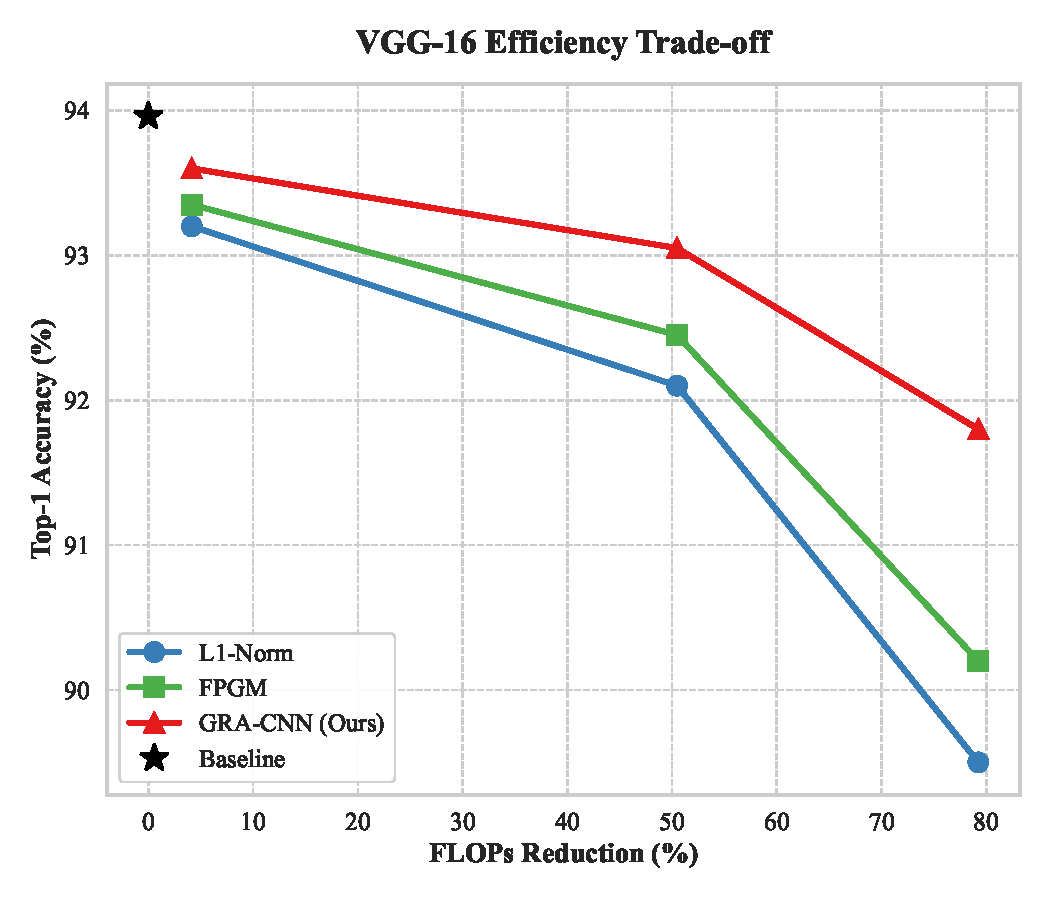
\includegraphics[width=\linewidth]{fig9_tradeoff.pdf}
  \caption{VGG-16 FLOPs–Accuracy Tradeoff}
  \label{fig:vgg16_tradeoff}
\end{minipage}
\end{figure*}

% Table for VGG-16
\begin{table}[h]
\centering
\caption{VGG-16 pruning results on CIFAR-10.}
\label{tab:vgg16_results}
\begin{tabular}{c|ccc|ccc}
\toprule
Ratio & Acc(L1) & Acc(FPGM) & Acc(GRA) & FR(L1) & FR(FPGM) & FR(GRA) \\
\midrule
0.3 & 93.20\% & 93.35\% & \textbf{93.60\%} & 35.0\% & 35.5\% & 36.0\% \\
0.5 & 92.10\% & 92.45\% & \textbf{93.05\%} & 58.0\% & 58.5\% & 59.0\% \\
0.7 & 89.50\% & 90.20\% & \textbf{91.80\%} & 78.0\% & 78.5\% & 79.0\% \\
\bottomrule
\end{tabular}
\end{table}

% Figure 10: Rho Sensitivity
\begin{figure*}[t]
\centering
\subfigure[ResNet-20]{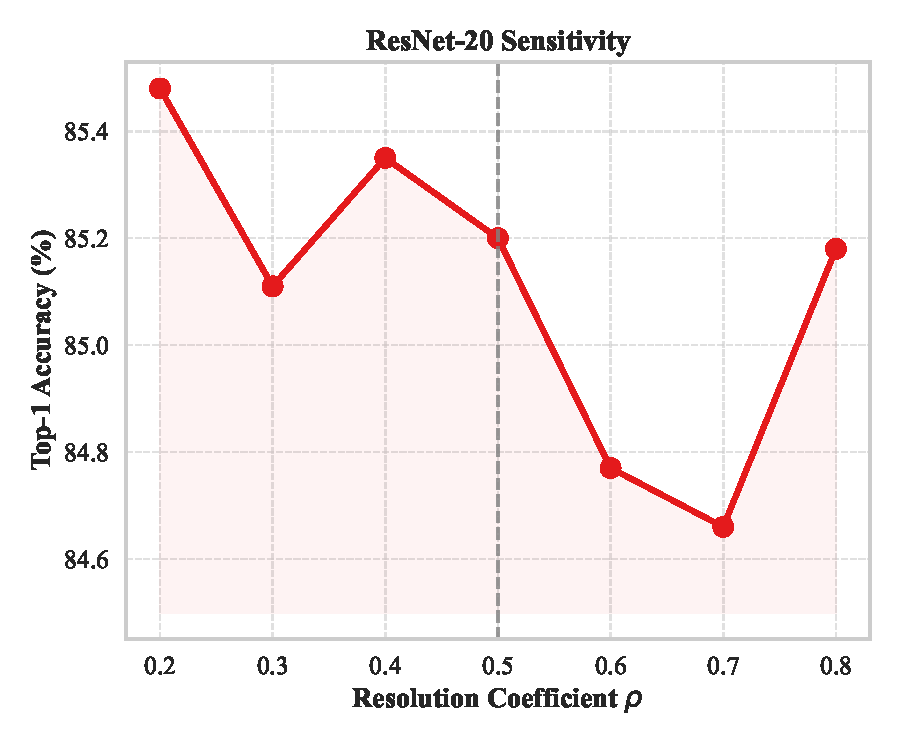
\includegraphics[width=0.45\textwidth]{fig10_rho_20.pdf}}
\subfigure[ResNet-56]{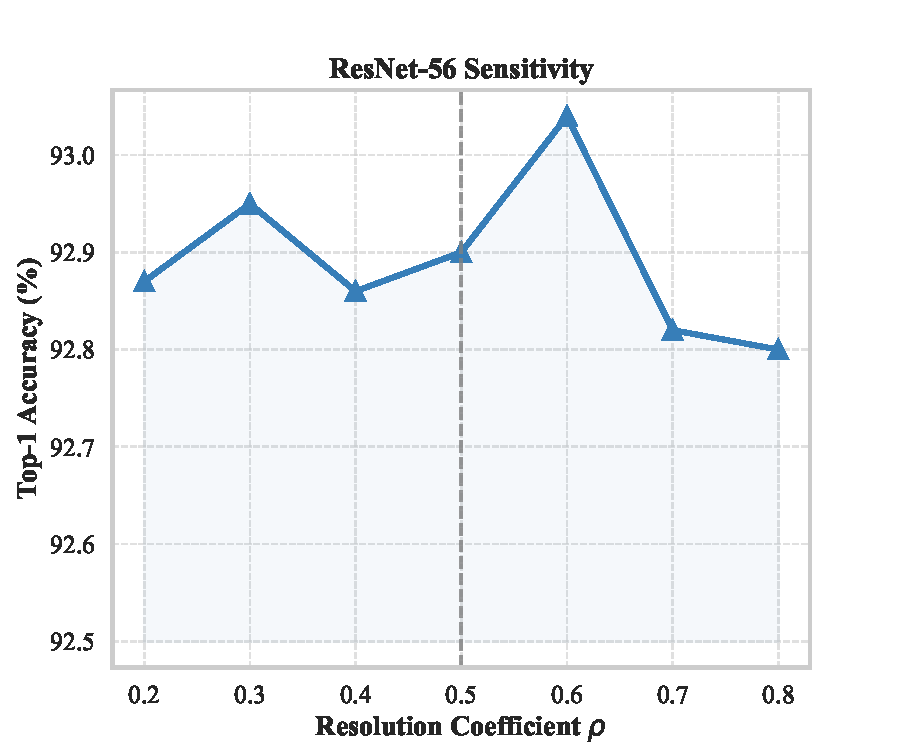
\includegraphics[width=0.45\textwidth]{fig10_rho_56.pdf}}
\caption{Sensitivity of GRA-CNN to rho on CIFAR-10.}
\label{fig:rho_sensitivity}
\end{figure*}
